% SPDX-License-Identifier: Apache-2.0
\documentclass[10pt,a4paper]{article}
\usepackage[margin=22mm,headheight=15pt]{geometry}
\usepackage{fontspec}
\setmainfont{Latin Modern Roman}
\setsansfont{DejaVu Sans}
\setmonofont{DejaVu Sans Mono}[Scale=0.82]
\usepackage{amsmath,amssymb,booktabs,array,tabularx,longtable,graphicx,float}
\usepackage[table]{xcolor}
\usepackage{microtype,enumitem,fancyhdr,titlesec,xurl,needspace,etoolbox}
\usepackage[most]{tcolorbox}
\usepackage{hyperref}
\definecolor{AlphaPurple}{HTML}{542BBC}
\definecolor{AlphaInk}{HTML}{192033}
\definecolor{AlphaMuted}{HTML}{596579}
\definecolor{AlphaLight}{HTML}{F3EFFA}
\definecolor{AlphaRed}{HTML}{922E44}
\hypersetup{colorlinks=true,linkcolor=AlphaPurple,urlcolor=AlphaPurple,citecolor=AlphaPurple,
 pdftitle={AGI ALPHA Flywheel: The Legal Work Advantage},pdfauthor={AGI ALPHA research contribution},
 pdfsubject={Executed synthetic legal-work support, capability reuse and conditional economics}}
\titleformat{\section}{\Large\sffamily\bfseries\color{AlphaPurple}}{\thesection}{0.65em}{}
\titleformat{\subsection}{\large\sffamily\bfseries\color{AlphaInk}}{\thesubsection}{0.65em}{}
\setlength{\parindent}{0pt}
\setlength{\parskip}{0.55em}
\setlength{\emergencystretch}{2em}
\renewcommand{\arraystretch}{1.23}
\setlist[itemize]{leftmargin=1.5em,itemsep=0.15em,topsep=0.3em}
\setlist[enumerate]{leftmargin=1.6em,itemsep=0.15em,topsep=0.3em}
\pagestyle{fancy}\fancyhf{}
\lhead{\small\sffamily AGI ALPHA · The Legal Work Advantage}
\rhead{\small\sffamily Research edition · 26 October 2026}
\cfoot{\small\sffamily\thepage}
\renewcommand{\headrulewidth}{0.3pt}
\newcolumntype{Y}{>{\raggedright\arraybackslash}X}
\newcommand{\money}[1]{\text{CAD }#1}
\newcommand{\evidence}[1]{\texttt{\small #1}}
\pretocmd{\section}{\Needspace{11\baselineskip}}{}{}
\pretocmd{\subsection}{\Needspace{7\baselineskip}}{}{}
\newtcolorbox{findingbox}[1][]{colback=AlphaLight,colframe=AlphaPurple,boxrule=0.5pt,arc=2mm,left=3mm,right=3mm,top=2mm,bottom=2mm,#1}
\begin{document}
\begin{titlepage}
\sffamily
{\small\bfseries\color{AlphaPurple} AGI ALPHA FLYWHEEL\hfill SUCCESSOR $\Omega$\par}
\vspace{20mm}
{\fontsize{35}{39}\selectfont\bfseries\color{AlphaInk} The Legal Work\\Advantage\par}
\vspace{8mm}
{\Large From bounded legal-work support\\to financeable capability growth\par}
\vspace{6mm}
{\large An executed study of source-linked contract packets,\\retained capabilities and commercial viability\par}
\vspace{12mm}
\begin{findingbox}
\textbf{Research verdict}\par
Exact text reconciliation passed its fresh technical checks. The broader playbook offering did not qualify, and no self-financing commercial flywheel was demonstrated.
\end{findingbox}
\vspace{5mm}
\begin{tabularx}{\textwidth}{@{}YY@{}}
\textbf{24 + 8} first-prototype cases & \textbf{12} additional fresh reconciliation cases\\
\textbf{2/24} complete primary packets for B, C1 and C & \textbf{12/12} exact-conservation packets for each ordinary comparison method\\
\textbf{0} additional complete packets from retained assets & \textbf{0/216} simulated worlds financing a first or second operating-funded investment\\
\textbf{CAD 0} actual collections & \textbf{Unknown} professional acceptance and complete actual cost
\end{tabularx}
\vfill
{\small AI-assisted research contribution coordinated through MontrealAI/AGI-Alpha-Agent-v0 issue \href{https://github.com/MontrealAI/AGI-Alpha-Agent-v0/issues/4850}{\#4850}. Independent construction and checking here mean separate agents within this research session; no qualified external legal reviewer or customer pilot was provisioned.\par}
\vspace{5mm}
{\small Original synthetic documents only · English contracts · English/French demonstration\\
TRANSFORMATIONAL INTELLIGENCE $\infty$ · Applicable \$AGIALPHA utility remains separate from operating earnings\\
26 October 2026 · Source and evidence edition for normal review}
\end{titlepage}

\section*{What was established}
\addcontentsline{toc}{section}{What was established}
\begin{tabularx}{\textwidth}{@{}>{\raggedright\arraybackslash}p{0.33\textwidth}Y@{}}
\toprule
\textbf{Commercial question} & \textbf{Executed evidence and limit}\\
\midrule
What useful work did a buyer receive? & No real buyer was onboarded. The research deliverable is a runnable source-bound comparison packet: both complete documents, exact changes, hashes, separate amendments and a professional review queue. The narrower technical contract passed on 12 fresh pairs with each of two methods.\\
What would competent human-only delivery require? & Counsel would use ordinary document comparison, inspect context and amendments, apply an organizational playbook, resolve ambiguity and make the final decision. That complete workflow was not timed; ordinary software must be included in the baseline.\\
What did AGI ALPHA cost, including necessary review? & Local generation and packaging subtotals were measured. Review, correction, integration, support, authoring and complete inference costs were not measured. Complete actual cost is unidentified; declared CAD scenarios are separate.\\
What capability was retained? & A definition/reference resolver and an explicit whole-clause amendment resolver, with source identities, scope, motivating development jobs, evidence and preserved failures.\\
How did the next unfamiliar job improve? & The first resolver corrected five additional rule statuses across three fresh cases. Complete accepted packets remained 2/24. The amendment addition produced no further primary gain.\\
Did surplus finance another improvement? & No actual collections occurred. None of 216 tested economic worlds funded a first or second capability from earned surplus. No second worthwhile investment was established.\\
\bottomrule
\end{tabularx}

\textbf{Abstract.} We built and executed a bounded legal-work support prototype using the existing portable AGI ALPHA SUCCESSOR Workbench, source-coverage machinery, unfunded Jobs compilation, and inherited capability-admission and accounting modules. The initial offering compared synthetic Ontario commercial mutual NDAs against an eight-rule research playbook. Source was frozen before a separate agent authored 24 primary cases and eight stresses. The baseline B, retained reference capability C1 and further amendment capability C each accepted 2/24 complete primary packets; an independently authored conventional implementation D accepted 0/24. C1 increased correct rule statuses from 125 to 130 of 192 without improving complete acceptance. A justified second prototype, frozen before 12 new cases, achieved exact text conservation in both ordinary character and line comparisons. These results establish bounded technical delivery, not legal correctness, useful localization or human-time savings. A corrected, separately frozen finite-cash model ran nine scenarios with 24 paired worlds and five strategies. Every reinvestment-world cash net result was negative; no operating-funded capability was purchased. Actual collections are zero and full actual costs remain unknown. The desired commercial succession is not established.

\textbf{Résumé.} Nous avons construit et exécuté un prototype d’assistance limité à des accords de confidentialité commerciaux synthétiques en Ontario. Seuls 2 dossiers sur 24 ont satisfait à l’ensemble des critères techniques du premier prototype pour les méthodes B, C1 et C. Une capacité conservée a corrigé cinq classements supplémentaires sans accroître le nombre de dossiers complets acceptés. Un second prototype de comparaison textuelle a conservé exactement les 12 nouvelles paires de documents, avec chacune des deux méthodes classiques. L’acceptation professionnelle, l’utilité du surlignage, le gain de temps humain et la viabilité commerciale ne sont pas établis. Aucune des 216 réalisations simulées n’a financé une première ou une deuxième capacité à partir d’un surplus d’exploitation. Les encaissements réels sont nuls; les coûts réels complets restent inconnus.

\section{The proposed purchase and its boundary}
\subsection{A recurring professional job}
The buyer hypothesis is an Ontario-qualified in-house commercial lawyer at a B2B software business who receives revised mutual NDAs during recurring business discussions. Each arrival creates a concrete decision: which changes require attention, which supplied policy conditions are satisfied, which questions remain unresolved, and what the lawyer should approve or change. Actual monthly workload, acquisition channels and willingness to pay were not observed. The repeated jobs here are an authored research workload.

The initial complete support packet includes original and revised text, document hashes, exact changed passages, in-scope obligation passages, eight playbook classifications, source references, unresolved amendments and a review queue. No packet constitutes an accepted agreement. No free-form revisions were ultimately produced. Client-specific strategy, enforceability, negotiation, signing and final legal acceptance remain with the qualified professional. Their labor is a material part of any proposed service, even when the provider does not directly pay for it.

Four candidate families were screened against usefulness, source checkability, recurrence, bounded review burden, alternatives, transferable work and complete cost. The initial budget allowed four families, at most two prototypes, two retained assets and no paid expenditure. Selection costs remain research costs even when not monetarily identified.

\begin{table}[H]\small
\begin{tabularx}{\textwidth}{@{}p{0.19\textwidth}YYY@{}}\toprule
\textbf{Candidate} & \textbf{Recurring trigger / output} & \textbf{Material remaining work} & \textbf{Disposition}\\\midrule
Playbook support & New NDA revision; deviations, obligations, source-linked review packet & Context, interpretation, acceptable revisions and final professional judgment & First prototype; 2/24 complete technical passes; service unqualified.\\
Version reconciliation & New draft pair; exact change and source packet & Determine significance and amendment effect; assess usability against ordinary tools & Second prototype; technical conservation passed.\\
Obligation tracking & Executed contract or amendment; dated register and alerts & Validate legal effect, triggers, ownership and continuing source updates & Not prototyped within budget.\\
Defined legal-change monitoring & Official source update; source-grounded change digest & Determine applicability, jurisdiction and required action; ongoing legal freshness & Not prototyped within budget.\\\bottomrule
\end{tabularx}
\caption{Qualitative discovery decisions, not observed market demand or scored customer preferences.}
\end{table}

The strongest practical alternatives matter. Microsoft Word already compares two versions and displays changes in a third document, with comparison options; it belongs in a competent human-only workflow \cite{word}. Spellbook documents reusable redline playbooks and tracked review workflows \cite{spellbook}. Neither product was executed here. D is an independent ordinary implementation, not a measured proxy for the strongest commercial legal software. The study therefore cannot establish competitive superiority.

\subsection{Jurisdiction and lawful support}
The initial scope is English-language, plain-text, commercial mutual NDAs in Ontario, Canada. The eight-rule playbook is an authored research policy, not Ontario law or a counsel-approved template. Ontario's Law Society Act restricts practising law, providing legal services and holding out, subject to its statutory and by-law exceptions; a licensee must remain within the licence's permitted scope \cite{lsa}. Efficiency does not supply authorization to practise.

The Law Society of Ontario's published generative-AI guidance addresses competence, confidentiality, candour, supervision, reasonable charges and tribunal duties. It calls for independent human verification of information relied upon and preservation of professional judgment \cite{lso}. Accordingly, the audience is qualified counsel using bounded support. No real-client material, privileged information, advice, filing, negotiation, external client communication or binding decision was undertaken. Public primary legal sources were checked on 26 October 2026. This limited research boundary is not a comprehensive regulatory opinion for commercial deployment.

The cases are original synthetic documents released with the original project code under Apache-2.0. They are marked as research documents and not for execution. No confidential intake is offered. Office format fidelity, OCR, consumer and employment contracts, privacy compliance, tax, securities, patent ownership and foreign legal interpretation are out of scope. The French demonstration translates the interface and findings, not the English contract corpus.

\section{Why earlier legal-productivity evidence is motivation}
Schwarcz and colleagues studied upper-level law students working with no AI, Vincent AI (2024), or o1-preview in an October 2024 experiment. Of 153 enrolled participants, 137 completed at least one task and 125 completed all six. Randomized stable groups assigned two tasks per condition. Three coauthors with legal practice experience graded work blind to condition and participant identity on five seven-point dimensions; time was self-reported. Productivity divided the sum of quality scores by the fraction of allotted time used. The NDA-drafting task did not show statistically significant quality, speed or productivity improvement \cite{schwarcz}. The study concerns assisted professional-style tasks, not autonomous agents, accepted client delivery, commercial demand or provider surplus. Its overall productivity findings justify investigation while leaving the commercial mechanism tested here unresolved.

\section{Executed system and evidentiary design}
\subsection{Reuse of the actual implementation}
The scientific Alpha source pin is \path{882456afe59d7bf9493ceaefc79f4f05c0cf7c9a}. We retained exact upstream files and license notices in a source manifest and extended the unchanged portable SUCCESSOR Workbench. A Python stage performs bounded parsing, policy checks and packet preparation. An in-process JavaScript adapter verifies document hashes and exact Unicode code-point spans, executes the native Workbench packaging path and retains its evidence receipt. The initial prototype also invokes the existing TRANSFORMATIONAL INTELLIGENCE source-coverage instrument. That structural instrument is not legal reasoning or independent legal verification.

An attempted native callback that spawned Python timed out at 45 seconds; a minimal diagnostic reported \texttt{EPERM}. The failed source and receipt are retained. The supported workflow is therefore explicitly two-stage: authorized local analysis, followed by in-process native verification and packaging. No execution restriction was bypassed. The signed-operator Harness and Fleet were not provisioned or executed.

Native packs remain \texttt{HOLD}, with empty active authority and \texttt{NOT\_CONNECTED} settlement. Seven existing Jobs work-order descriptions are compiled per pack; they are unfunded descriptions, not executed or settled commercial jobs. Fleet, Jobs and Manager were source-audited at the pins in Appendix~\ref{app:reproduce}; their validators, contracts and settlement were not changed. The research uses Python 3.12 and Node 24.22.1. It does not claim qualification under the repository's pinned Node 22.17.1 release profile.

\subsection{The compared methods}
\begin{table}[H]\small
\begin{tabularx}{\textwidth}{@{}p{0.08\textwidth}YY@{}}\toprule
\textbf{Arm} & \textbf{Implemented or specified workflow} & \textbf{What it can identify}\\\midrule
A & Competent human-only work with normal non-AI comparison and research tools; not executed & Workflow requirements and conditional wage-based resource cost; no measured human-time advantage.\\
B & Newly built conventional regex/diff adapter & Initial authored implementation, not a historical deployed NDA service.\\
C1 & B plus retained definition/reference resolver & Incremental effect of the first asset on frozen fresh work.\\
C & C1 plus explicit whole-clause amendment resolver & Incremental effect of the second asset.\\
D & Separately authored conventional parser with the same task specification and ordinary methods & An independent engineering comparison; not Word, Spellbook or best available legal AI.\\
T & A separate invocation of acquired C code & Executable transfer; not proof of a recipient's prior incapacity or a unique reasoning method.\\\bottomrule
\end{tabularx}
\caption{Human-work advantage, competitive positioning, incremental asset value and unique-method advantage are separate questions.}
\end{table}

D was first constructed without C's source. Subsequent shared integrity review found duplicate amendment targets and ignored operative text; both implementations received the same criticism before fresh confirmation. The original D and failed construction history were preserved. This review reduces strict implementation isolation but improves fairness of the final integrity boundary. All arms remain small deterministic systems authored by agents; results should not be generalized to frontier model-assisted legal review.

\subsection{Acceptance and severity}
Eight policy families were declared: permitted purpose, confidentiality term, return deadline, compelled-disclosure notice, residuals, assignment, governing law and representatives. Six receive research severity 5 and two severity 3. The duration and notice thresholds are experimental policy choices. Each rule has a status among pass, deviation, absent, uncertain and out of scope, with exact supporting passages.

Complete acceptance requires the scoped statuses and required supporting/obligation passages to agree with the independent synthetic key, exact source references, complete changed-text coverage, visible escalation and no unsupported revision. No severity-5 false pass is permitted. A weighted status error sums the severity of each incorrect classification, so many correct trivial checks cannot erase a material error. The primary denominator is $24(6\cdot5+2\cdot3)=864$ severity units. Independent legal correctness, appropriate drafting, preservation of intended legal meaning and customer acceptance are different endpoints and were not assessed.

The source/checker freeze preceded case generation. A separate agent who did not read B/C/D authored 24 primary cases and eight distinct stresses, covering unfamiliar language, cross-references, definitions, amendments, conflicts, missing provisions and out-of-scope questions. Keys and private annotations were outside production inputs, skill records and retrieval. All 160 predictions were sealed before key release: 96 primary B/C1/C/D comparisons, 32 separate stress comparisons and 32 T invocations. Source files were not repaired after outcomes.

These are a small purposively varied synthetic cohort and same-session agent annotations, not a random sample of customer contracts or external legal adjudication. Mechanical completeness has stronger evidence than domain validity. Subsequent stricter document-scoped change auditing addressed a frozen scorer weakness concerning amendment offsets; it changed no accepted-packet outcome. That audit is supplementary and does not replace the original frozen score.

\section{First prototype: partial improvements did not qualify the service}
\begin{table}[H]\small
\begin{tabularx}{\textwidth}{@{}lrrrrY@{}}\toprule
\textbf{Arm} & \textbf{Complete} & \textbf{Rules} & \textbf{Weighted error} & \textbf{False passes} & \textbf{Required support / obligations covered}\\\midrule
B & 2/24 & 125/192 & 281/864 & 1 & 183/204; 181/190\\
C1 & 2/24 & 130/192 & 256/864 & 1 & 187/204; 181/190\\
C & 2/24 & 130/192 & 256/864 & 1 & 187/204; 181/190\\
D & 0/24 & 116/192 & 328/864 & 1 & 163/204; 157/190\\\bottomrule
\end{tabularx}
\caption{Primary mechanical results. All four arms missed the same severity-3 representatives-responsibility issue. Professional acceptance is unknown in every case.}
\end{table}

\begin{figure}[H]\centering
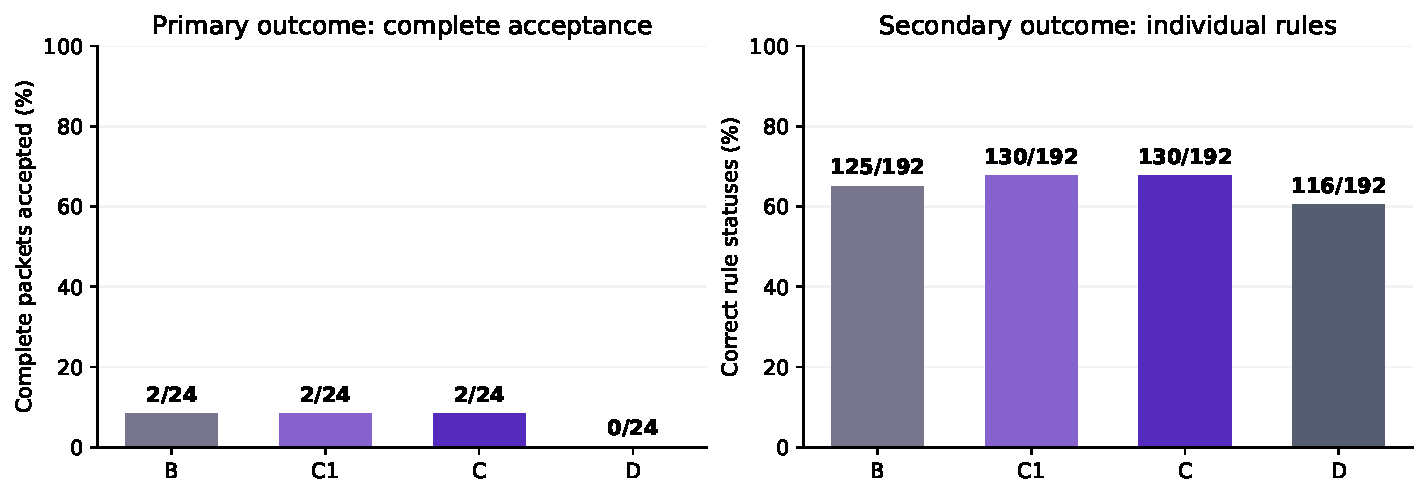
\includegraphics[width=\textwidth]{figures/primary-acceptance.pdf}
\caption{Correct individual classifications did not translate into a dependable complete packet. All methods used the same 24 cases; each case contains eight research policy rules. These counts are not lawyer-validated legal accuracy.}
\end{figure}

C1 added five correct rule statuses across PRIMARY-09, PRIMARY-10 and PRIMARY-12. In PRIMARY-09, the obligation referred to a ``Protection Interval'' and a separate definition stated ``thirty months.'' B returned uncertainty. C1 linked the obligation to that definition and correctly classified the authored 12--36-month policy as satisfied. It likewise resolved a separately defined 28-calendar-day return interval. PRIMARY-10 contained 42-month and 35-day cross-references; C1 correctly identified those policy deviations. This is an inspectable retained executable capability improving fresh subproblems \cite{primaryrun}.

However, B, C1 and C accepted only PRIMARY-17 and PRIMARY-20 as complete primary packets. These two technical passes include correctly reported absences and unresolved terms: acceptance means that the support packet matches the declared key and surfaces its review questions, not that the agreement is complete, legally acceptable or ready to sign. The amendment resolver added no primary classification or acceptance gain. Common wording still failed: return obligations phrased as ``returned or destroyed'' could be missed, and consent expressed through ``only after receiving'' could remain uncertain. Every arm falsely passed the representatives-responsibility issue in PRIMARY-08. No severity-5 primary false pass occurred, but that narrower observation must not conceal the severity-3 miss or incomplete obligation extraction.

All 160 outputs passed exact-reference and changed-character conservation checks, including the stricter supplementary audit. No proposed revisions were emitted. Consequently, zero unsupported revisions is an abstention result, not evidence of correct legal drafting. Many conservative uncertainties prevented acceptance; over-escalation can still consume expensive professional review.

The separate stress cohort accepted B/C1/C in 3/8 cases and D in 4/8. T was identical to C on all 32 tested cases. A post-freeze development diagnostic also exposed a same-sentence amendment problem: text following a precedence phrase could be swallowed even when it introduced an additional operative change. The source and diagnostic are retained without primary repair. They restrict the asset's supported claims rather than being erased by aggregate accuracy.

Mean measured Python-plus-native production subtotals were 0.11368 seconds for B, 0.10372 for C1, 0.10111 for C and 0.10198 for D. These subtotals include local analysis and output preparation plus Workbench execution/inspection, but exclude some batch serialization/startup, later key scoring and all professional work. Subsequent independent scoring took 9.465 seconds across 160 packets. Neither tiny runtime differences nor automated check counts establish an accepted-service cost advantage.

\section{Second prototype: exact reconciliation on new work}
The initial offering failed for reliability and unresolved review burden. Within the original two-prototype limit, we narrowed the deliverable to exact plain-text version reconciliation with separate, uninterpreted amendments. This is a different technical product and a separately reported experiment. It removes unsupported semantic claims; it does not silently remove necessary legal review from a complete service.

The new source, scope and independent conservation checker were frozen before 12 further cases were authored: two each for sentence edits, insertion/deletion, movement/renumbering, separate amendments, Unicode/formatting and nested/cross-reference changes. The two actual methods are character and line \texttt{SequenceMatcher} comparisons. There is no additional retained asset and no fabricated B/C efficacy replication. All 24 outputs were sealed before the new keys were released.

The independent checker binds the packet to the original intake documents, verifies hashes and operation labels, reconstructs both entire texts from contiguous ordered spans and preserves every separate amendment. It does not use the producer's diff algorithm. Alternative valid alignments are accepted. This makes the criterion reproducible, but also means that a whole-document replacement could pass while being a poor review aid.

\begin{table}[H]\small
\begin{tabularx}{\textwidth}{@{}Yrr@{}}\toprule
\textbf{Fresh result} & \textbf{Characters} & \textbf{Lines}\\\midrule
Exact-conservation packets & 12/12 & 12/12\\
Operations / changed operations & 116 / 53 & 39 / 17\\
Original highlighted code points & 788 & 3,528\\
Revised highlighted code points & 892 & 3,632\\
Unchanged revised context & 90.18\% & 60.00\%\\
Separate amendments preserved & 4 & 4\\
Mean local production subtotal & 0.04619 s & 0.03340 s\\
Professional / usability acceptance & Unknown & Unknown\\\bottomrule
\end{tabularx}
\caption{The same 12 new pairs, totaling 8,976 original and 9,080 revised code points. Smaller highlighted volume is descriptive, not a demonstrated human review benefit.}
\end{table}

For example, RECON-01 adds use of supplied records to build an internal proof of concept to a business-evaluation sentence. The packet displays the deleted and added text in that replacement, together with both complete source documents. It makes no conclusion about whether that change is acceptable. RECON-07 and RECON-08 retain two amendments each without inferring precedence or a consolidated agreement. RECON-09 and RECON-10 preserve Unicode distinctions and formatting. The interface lets the reader inspect both granularities and the evidence boundary \cite{reconrun}.

The narrower product has a functioning auditable output and technical acceptance. It has no demonstrated advantage over already available ordinary comparison tools, no measured professional time saving, no buyer validation and no professionally accepted legal outcome. We therefore stop the bounded discovery rather than continue polishing a commercially unvalidated workflow.

\section{Retention, transfer, sharing and change}
\subsection{What was actually retained}
The reference asset originated in DEV-03 and DEV-04, where defined periods and cross-references defeated local matching. The amendment asset originated in DEV-05. Their source identities, construction motivation, scope, version, validation and failures are recorded in \path{evidence/capability-history.json}. The first asset's five fresh classification improvements are real within the authored policy; no complete-packet or human-effort gain follows automatically.

T demonstrates that another invocation can acquire and execute C. It does not demonstrate that a competent recipient lacked the capability before acquisition. D independently reconstructed an ordinary solution with access to the task and normal tools; its weak primary result is not proof of inability after all reasonable reconstruction. No rare-capability claim or exclusive method advantage is justified. Complete construction/inference cost was not metered, so the paper does not describe the retained code as free.

\subsection{Equal inventory registry and graph}
The sharing panel imports the prior authority, commitment and selection modules unchanged. Direct retention, indexed registry and graph-guided reuse receive the same two assets, evidence and one dependency. Registry and graph both validate the shared root and perform the same 12 proof checks, two attestation checks, one root-authority check, 11 reads and 122,655 hashed bytes per selection. No artificial registry search delay is imposed \cite{graphdata}.

\begin{table}[H]\small
\begin{tabularx}{\textwidth}{@{}Yrrr@{}}\toprule
\textbf{Selection method} & \textbf{Repetitions} & \textbf{Mean wall ms} & \textbf{Mean CPU ms}\\\midrule
Independent direct recipe & 50 & 1.509 & 1.602\\
Shared searchable registry & 50 & 5.769 & 6.433\\
Graph-guided reuse & 50 & 5.557 & 6.504\\\bottomrule
\end{tabularx}
\caption{All select the same two assets. Direct retention does not validate a shared root and therefore provides different guarantees. Two assets and these small timing differences establish no graph-specific commercial advantage.}
\end{table}

The admission scope is exact source fidelity and composition on six development documents, not legal correctness. The existing research SHA-256 Merkle and proof-loop machinery is used within its stated canonicalization. It is not asserted to match a deployed Solidity ABI or live on-chain proof. Attestation fixtures use eligible-form \texttt{*.agent.agi.eth} names, with separate issue-attestation and commit-root operation grants. They are not authenticated accounts. LIVE admission refuses without authenticated eligible identity. Existing AGI Jobs \texttt{*.club.agi.eth} validation, contracts and settlement remain unchanged.

\subsection{Obsolescence and upkeep}
Twenty-one adverse controls refuse invalid current reuse, including changed jurisdiction, playbook, law-epoch marker, format, host/source/dependency identity, expiration, revocation, role separation and invalid rollback. The historical fixture root cannot authorize a changed current scope. Earlier versions and failed instrumentation remain available. These are executable freshness and identity controls, not an experiment observing an actual change in Ontario law or measuring a lawyer's revalidation time.

Reference and amendment assets remain research source, with legal admission unqualified after the fresh results. New legal conclusions would require independent professional validation and renewed current-scope evidence. Human revalidation cost and useful commercial lifetime are unknown. Economic sensitivity charges declared upkeep; it cannot establish that actual maintenance will fit within reuse savings.

\section{Cost accounting and commercial simulation}
\subsection{Observed resources and unidentified costs}
Local execution measurements and actual collections must be distinguished from monetary assumptions. The full accounting boundary includes discovery, public legal research access, authoring/inference, development failures, parsing, analysis, verification, rejected attempts, correction, packaging, necessary professional review, integration, acquisition, support, maintenance and capability revalidation. No invoice-level measurement of all those categories was available.

\begin{table}[H]\small
\begin{tabularx}{\textwidth}{@{}p{0.24\textwidth}YY@{}}\toprule
\textbf{Cost layer} & \textbf{Observed in this run} & \textbf{What remains unknown or assumed}\\\midrule
Marginal production & Per-attempt generation/check/packaging subtotals, including rejected packets & Compute tariff, inference/authoring allocation, handling and professional correction.\\
Recurring service & No real customers or paid service recurrence & Research subscriptions, support, customer integration, acquisition, legal review and ongoing maintenance.\\
Fully allocated & Historical failures, sources and development artifacts retained & Complete research cost, human attention, full overhead and historical recovery.\\
Cash and obligations & Actual customer collections and financial transactions: zero & Complete actual cost and available earned surplus: unidentified.\\
Capability investment & Two executable assets and their validation/failure history & Actual construction and revalidation money; CAD scenario allocations are not invoices.\\\bottomrule
\end{tabularx}
\caption{Missing costs are null/unknown, not zero. The companion retains a full-category ledger and the raw resource observations.}
\end{table}

The Government of Canada Job Bank reports an Ontario lawyer employee median of CAD65.21/hour, with CAD32.05 and CAD112.98 low/high values for the cited wage period \cite{jobbank}. This is not a billing rate. The model's 1.3 employment burden, 45-minute human task, review minutes and all service-specific times are explicit sensitivity coordinates, not measured task durations or calibrated willingness to pay. A vendor NDA-spotting benchmark is retained only as contextual literature; it is not converted into an accepted Ontario packet estimate.

\subsection{The finite-cash model}
We reused the canonical shadow ledger and buyer-choice primitives from the preceding study. The corrected model runs nine declared scenarios, 24 paired seeds and five strategies over 26 weeks: continued B, seed-funded C1, seed-funded C, a conventional improvement D, and contingent reinvestment. The 96 primary B/C1/C/D records supply observed technical outcomes and runtime. Stress and T records do not calibrate the market. The model has finite cash, a CAD2,000 seed and CAD200 reserve; seed is never counted as earned surplus. Throughout this report, simulated cash net result means simulated collections less all modeled provider cash costs, including newly purchased capability construction. Seed is excluded; unknown historical and complete actual costs remain unidentified. This is not accrual operating profit or observed earnings.

Reference assumptions include 12 prospective buyers, 0.4 weekly arrival probability, CAD10 offered price, CAD2 acquisition cost on each arrival of a not-yet-onboarded prospect (including repeated declined visits), one hour of provider onboarding at CAD40/hour, one hour of buyer onboarding allocated over 12 assumed jobs, four operator minutes and one support minute per attempt, CAD0.25 tools per attempt, CAD5 fixed weekly cost and CAD2 weekly maintenance. A generic competitor costs an assumed CAD3 plus 20 minutes of review; this is not a vendor quote. The buyer may decline and choose an alternative. Only an assumed 50\% of capacity value is realized in buyer utility; avoided payroll cash is zero by default.

The sensitivity rows are bundled scenarios, not isolated causal effects. The lower-price row also assumes 15-minute review. The correction row adds ten correction minutes to that bundle. The no-buyer-onboarding row removes buyer onboarding from the correction bundle; higher-repeat work additionally raises arrival probability to 0.8. Higher maintenance instead combines 15-minute review, CAD5 price and ten correction minutes with CAD20 weekly upkeep while retaining buyer onboarding. The exact parameter file defines every bundle.

Professional acceptance is an unobserved conditional assumption of 0.95 after technical acceptance. Collection probability is assumed 0.98 with a two-week delay. Only sampled packets already passing the deterministic gate may become invoices under the conditional acceptance draw. Hypothetical correction effort remains a cost and never changes a failed production row into an accepted one. Obligations, reserve and unpaid receivables are distinct from collected money. No token issuance, price appreciation or \$AGIALPHA balance contributes operating earnings \cite{economicrun}.

An initial model defect allowed invoices for rejected packets. Its diagnostic produced 115 such invoices in one scenario; that result is explicitly invalid and preserved. The v2 repair froze before the valid campaign and kept all scenario parameters and seeds unchanged. Independent audit reconciled 1,080 stored strategy summaries with 13,403 assertions and found no arithmetic discrepancy. One high-attempt world was replayed to reconcile weekly cash and invoice delays. A stale v2 explanatory sentence and optimistic buyer-perceived quality assumption are documented errata: technical quality gates actual invoicing, while the demand model still uses optimistic assumed quality rather than measured overall success. No post-outcome favorable retuning was performed.

\subsection{Resource cost, customer savings and price}
At the declared burdened wage, the hypothetical 45-minute human workflow costs CAD63.58 in employee opportunity cost. The unit table displays CAD3.59 provider marginal cost per B attempt before unknown full costs, and the buyer still bears CAD63.58 of assumed review. CAD10 price plus CAD7.06 allocated buyer onboarding produces CAD80.64 of buyer price-and-attention cost. These resource-cost comparisons value capacity at the full assumed loaded wage; primary buyer choice separately applies 50\% capacity realization. Neither is measured willingness to pay or avoided payroll. This comparison is unfavorable under the no-time-benefit assumption; it is not an actual invoice comparison. The unit table separately rounds labor components; the cash campaign rounds combined labor and charges CAD3.58 for the corresponding B attempt. The one-cent display difference is disclosed rather than silently reconciled by changing frozen results.

If the authored 2/24 technical acceptance fraction were a future attempt frequency, the displayed CAD3.59 per attempt would imply CAD43.08 per technically accepted packet (CAD42.96 using the cash campaign's CAD3.58 rounding), even before missing recurring costs. That conditional arithmetic is not a validated production forecast. Compute can round to zero cents at the model's small tariff while raw positive runtime remains recorded. No token-cost-versus-lawyer-invoice advantage is claimed.

For narrow reconciliation, ordinary comparison may already be licensed. With a fee $p$, added integration $i$ minutes and opportunity-cost wage $w$, the necessary saved professional minutes are
\[
\Delta t_{\min}=\frac{60p}{w}+i,\qquad w=65.21\times1.3=\money{84.773}\text{/hour}.
\]
CAD5, CAD10 and CAD20 require respectively 3.54, 7.08 and 14.16 saved minutes before integration. At CAD10 and one additional minute, the threshold is 8.08 minutes. No such saving was observed. The frozen secondary analysis uses only the two real methods, equal assumed review effort, 1/3/5/10/20-minute ordinary review coordinates, and separate handling/onboarding cost sensitivities. It does not create duplicate B/C arms or claim a new capability.

\section{Operating surplus and reinvestment results}
All 216 reinvestment-world cash net results were negative. Reinvestment purchased neither the first nor second asset in any world and exactly matched continued B, because its investment conditions were not met. The reference generated zero modeled collections and mean 26-week simulated cash net result of $-\money{428.92}$; the 10th/90th scenario quantiles were $-\money{450.00}$ and $-\money{414.00}$. These are simulated distributions under declared assumptions, not empirical market confidence intervals.

\begin{figure}[H]\centering
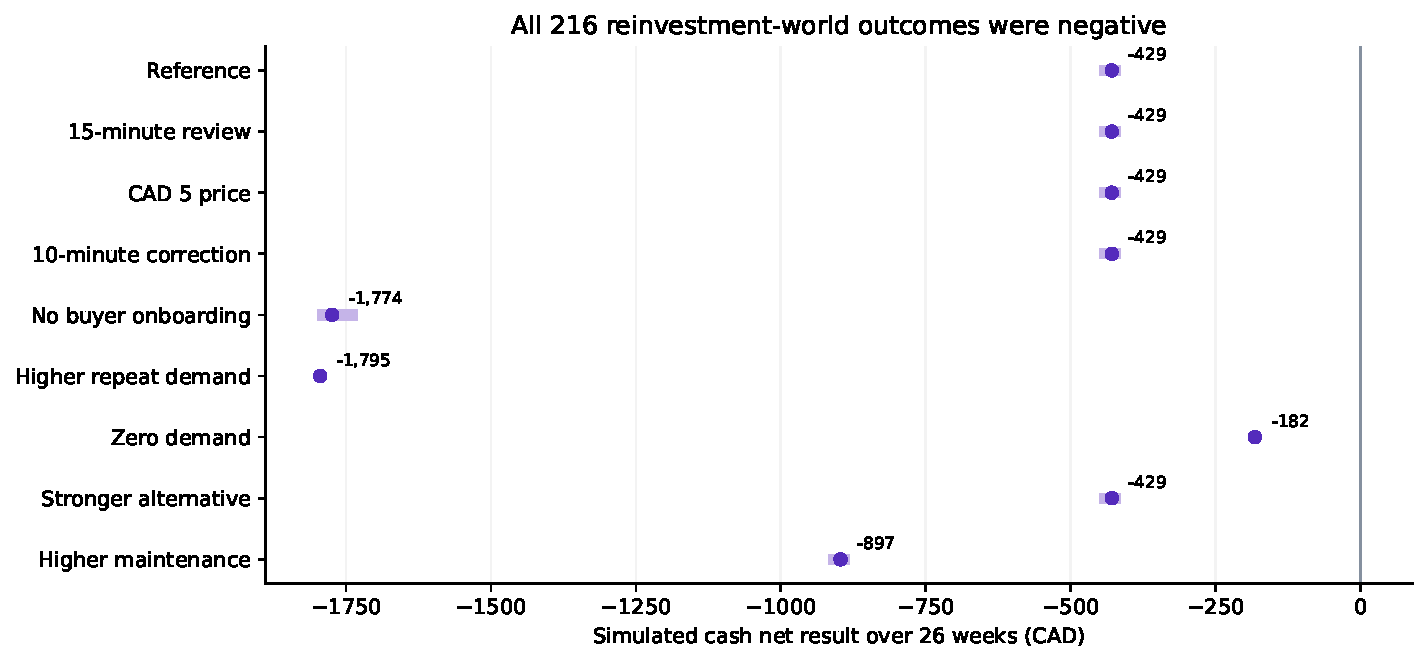
\includegraphics[width=\textwidth]{figures/economics-sensitivity.pdf}
\caption{Mean and 10th--90th scenario quantiles across 24 paired seeds per condition. No first or second operating-funded investment occurs. Some assumptions reduce modeled losses; none establishes commercial viability.}
\end{figure}

\begin{table}[H]\small
\begin{tabularx}{\textwidth}{@{}Yrrr@{}}\toprule
\textbf{Scenario} & \textbf{Mean cash net CAD} & \textbf{Mean collections CAD} & \textbf{First / second investment worlds}\\\midrule
Reference, no measured time benefit & $-428.92$ & 0.00 & 0 / 0\\
Conditional 15-minute review & $-428.92$ & 0.00 & 0 / 0\\
Conditional CAD5 price / review & $-428.92$ & 0.00 & 0 / 0\\
Conditional 10-minute correction & $-428.92$ & 0.00 & 0 / 0\\
No buyer onboarding & $-1{,}774.12$ & 47.08 & 0 / 0\\
Higher repeat work & $-1{,}794.63$ & 47.71 & 0 / 0\\
Zero demand & $-182.00$ & 0.00 & 0 / 0\\
Stronger lower-cost alternative & $-428.92$ & 0.00 & 0 / 0\\
Higher maintenance & $-896.92$ & 0.00 & 0 / 0\\\bottomrule
\end{tabularx}
\caption{Twenty-four paired worlds per row; rows are the bundled scenarios defined in the finite-cash model description, not isolated causal effects. The five-strategy histories, buyer flows, all contrasts and exact ledger records are preserved in the companion.}
\end{table}

More assumed demand is not automatically helpful when low acceptance produces many unreimbursed attempts. A checked high-repeat world contains 12 simulated customers, 134 attempts and 116 technical failures. It has 16 invoices, 15 paid collections totaling CAD75, costs CAD1,869.44, cash net result $-\money{1{,}794.44}$ and zero earned surplus. Closing cash CAD205.56 still includes the CAD200 reserve and residual seed. This is not money earned for reinvestment.

Some C-versus-D or C1-versus-B differences favor an asset in individual loss-making worlds. Those relative comparisons remain in the result files; they are not positive operating surplus, complete project repayment or an investment-qualified succession. The model's first asset allocation is CAD300 plus CAD100 failed construction, the second CAD400 plus CAD100 failed construction, with a 13-week assumed lifetime and charged upkeep. Historical research cost remains unknown and is not charged again as a measured prospective construction invoice.

For a candidate with prospective construction $K$, failed-attempt construction $F$, maintenance per use $m$ and actual incremental saving per use $s$, a finite direct-cost break-even requires $s>m$ and
\[
n_{\mathrm{BE}}=\left\lceil\frac{K+F}{s-m}\right\rceil.
\]
Repayment must occur before expiry and after interruption, adaptation, validation and business costs. With zero demonstrated incremental complete-packet benefit and no measured human-time saving, the tested no-benefit accounting condition has no finite payback. This is a conditional conclusion, not a claim that every future reuse can never pay. At an assumed CAD400 fixed cost and CAD0.25 upkeep, 50 uses require at least CAD8.25 gross saving per use to break even; 100 uses require CAD4.25. A positive return requires more. These savings have not been established. Actual lifetime and future law/playbook revalidation expense remain unidentified.

\section{Commercial disposition and the next decisive evidence}
The initial playbook-support offering is not qualified for sale as a complete review service. The narrower reconciliation prototype is technically functional, but is not established as worth purchasing against ordinary software. The work supports retaining its transparent source packet as a research asset and withholding a commercial success claim. A cheaper computation, a useful retained subroutine, an attractive complete service and a self-financing succession remain distinct achievements.

The next justified experiment would have to resolve the present value bottleneck rather than merely improve runtime. It would require appropriately qualified independent reviewers, a versioned counsel-approved playbook where semantic review is intended, and a matched normal-tool workflow. Record all intake, correction, review, integration and acceptance effort; test documents chosen before outcomes; compare ordinary comparison and a strong available AI-assisted product under the same deliverable standard. Buyers should face a concrete price and remain free to decline. Such work was not authorized as client onboarding or a paid engagement in this assignment and was not performed.

The decisive commercial test is whether an accepted support packet reduces complete professional effort enough to cover price and integration while preserving quality, and whether the provider collects enough after all costs, obligations and reserves to fund an independently worthwhile capability. Any later capability must then repay on fresh work versus continued delivery and a competent conventional improvement. The present run supplies an auditable starting implementation and failures, but it does not satisfy those conditions.

\appendix
\section{Reproduction, provenance and publication boundary}\label{app:reproduce}
The complete companion contains code, exact upstream dependencies, original synthetic inputs, released answer keys, all rejected and accepted research packets, native packs, economic model and histories, source/input/prediction freezes, failures, independent checks, figures, this LaTeX source and the self-contained EN/FR HTML replay. Answer keys are public in this final reproducibility edition; they were unavailable to production before sealing and are never imported by the producer or skill registry.

\begin{table}[H]\small
\begin{tabularx}{\textwidth}{@{}p{0.24\textwidth}Y@{}}\toprule
\textbf{Repository} & \textbf{Audited scientific source pin}\\\midrule
AGI-Alpha-Agent-v0 & \path{882456afe59d7bf9493ceaefc79f4f05c0cf7c9a}\\
AGI-Fleet-Linux & \path{45759fb096faf8988f58ae5ea71248d0f35a97c7}\\
AGIJobsv0 & \path{bc4abbd5c28f3672275b13300e40ea26c820b8ee}\\
AGIJobManager & \path{5d5670df9dbbc79da115e0a44b71989f34df58c1}\\\bottomrule
\end{tabularx}
\end{table}

\Needspace{11\baselineskip}
From the extracted companion root, using Python 3.12 and Node 24.22.1, run to new directories:
\par\vspace{0.3em}
\begin{minipage}{\textwidth}
\begin{verbatim}
python src/run_production.py --cohort primary --output replay/primary
node src/native_packaging.mjs replay/primary/packaging-manifest.json \
  replay/primary/native-records.json
python reconciliation/reconcile.py replay/reconciliation
node reconciliation/package.mjs replay/reconciliation/packaging-manifest.json \
  replay/reconciliation/native-records.json
\end{verbatim}
\end{minipage}
\par\vspace{0.3em}
The production runners refuse overwriting an existing campaign. Replays verify reproducibility and do not create new scientific samples or customers. The evidence index gives evaluator, economic and graph commands. Complete actual financial recovery cannot be reproduced from absent invoices; the model reproduces only its declared conditional world.

\begin{longtable}{@{}p{0.28\textwidth}p{0.68\textwidth}@{}}
\toprule\textbf{Custody record} & \textbf{SHA-256}\\\midrule\endhead
First source freeze & \path{7b4b0afed9861ed59d53e146d7b2d63b2ffb22a999d878344cb761000d6ad85b}\\
First prediction seal & \path{08e4ffb331dfed4177f0926ae19c4b0e2afd0af33454006258cba7566cc94622}\\
Second source freeze & \path{3f41122d1e89e8a42916816bd0aca90905b7b7edfd43ec552b6898c9531c09ae}\\
Second input freeze & \path{086a97337176a991715a3adbe59a2f30da4df6875ebf217d36c4089e9d2c2df5}\\
Second prediction seal & \path{6e048513e1b4773e0651bf22ed8aee1c407a16302d97757434681e76c15ed5d0}\\
Corrected economics source & \path{e441adeafc444247159dc849158ff6adf4cbaabcddc445aaa45307733aa82e7a}\\
Primary economics results & \path{059164d92544d45801fea6f025a6f87d0e7169cf1759ac02d7e95154f8db1c9e}\\\bottomrule
\end{longtable}

Publication is an additive source-review contribution under \path{studies/agi-alpha-legal-work-v1/}. Existing studies, negative findings, shared catalog, release owners and held operational paths remain intact. Local scoped checks do not replace required repository or hosted qualification. In particular, exact inherited and historical source can retain lint findings in its relocated research paths; frozen code is not silently reformatted, suppressed or renamed to evade those gates. Full repository setup/hooks, release qualification, installed adoption, browser visual acceptance and public hosting are not claimed by this paper. The final delivery receipt records the draft/source status and any unresolved checks separately from the scientific freezes.

\section{Evidence index and accounting notes}
\begingroup\small\renewcommand{\arraystretch}{1.1}
\begin{longtable}{@{}p{0.33\textwidth}p{0.63\textwidth}@{}}
\toprule\textbf{Question} & \textbf{Companion evidence}\\\midrule\endhead
Initial selection and professional boundary & \path{protocol/scope.json}; \path{research/legal-scope/evidence.json}; \path{research/legal-scope/final-boundary-notes.md}\\
Every original prediction and packet & \path{evidence/primary/}; \path{evidence/stress/}; \path{protocol/prediction-seal.json}\\
Complete acceptance and severity & \path{evidence/production-summary.json}; \path{evaluation/scorer.py}; \path{evaluation/audit_predictions.py}\\
New reconciliation confirmation & \path{reconciliation/}; \path{evidence/reconciliation/}; \path{evidence/reconciliation-independent-audit.json}\\
Retained assets and known defects & \path{src/references.py}; \path{src/amendments.py}; \path{evidence/capability-history.json}; \path{evaluation/independent-source-review.json}\\
Sharing, admission and change & \path{graph/catalog.json}; \path{graph/results/}; \path{graph/history/}; \path{graph/source-provenance.json}\\
Complete conditional economics & \path{economics/parameters.json}; \path{economics/results/primary-v2/}; \path{economics/results/reconciliation/}; \path{economics/findings.md}\\
Independent cash audit and errata & \path{evidence/economics-independent-audit.json}; \path{economics/history/model-v1/}; \path{economics/model-validity-diagnostic-v1.json}\\
Full cost categories and unknowns & \path{evidence/cost-accounting.json}; \path{economics/production-input.json}; canonical ledger events embedded in the campaign\\
Bilingual demonstration & \path{demo/AGI_ALPHA_Legal_Work_Demo.html}; \path{research/legal-scope/french-demo-review.md}\\\bottomrule
\end{longtable}
\endgroup

\Needspace{8\baselineskip}
Known failed construction and validation attempts include the native subprocess path, preconfirmation amendment defects, an original independent D version, a preserved post-freeze amendment edge case, preconfirmation reconciliation input/operation validation defects, a graph timing-instrumentation defect and the invalid first economic model. Their costs are not erased. Actual model inference and active human attention were not metered. The study cannot provide a truthful single all-in dollar total; its ledger marks that incompleteness explicitly. The prospective investment scenarios price construction once, retain failed-construction allocations and do not silently charge unknown historical research a second time.

\begin{thebibliography}{20}\small
\bibitem{schwarcz} D. Schwarcz, S. Manning, J. J. Prescott, P. Barry, D. R. Cleveland and B. Rich. \emph{AI-Powered Lawyering: AI Reasoning Models, Retrieval Augmented Generation, and the Future of Legal Practice}. Journal of Law and Empirical Analysis, 2026. \href{https://doi.org/10.1177/2755323X261427048}{doi:10.1177/2755323X261427048}. University repository: \url{https://repository.law.umich.edu/facarticles/3173/}. Methods, task-specific tables and limitations consulted; cited, not redistributed.
\bibitem{lsa} Ontario. \emph{Law Society Act}, R.S.O. 1990, c. L.8, especially ss. 1 and 26.1. Current e-Laws consolidation accessed 26 October 2026. \url{https://www.ontario.ca/laws/statute/90l08}. Statutory and by-law exceptions remain relevant; no deployment opinion is inferred.
\bibitem{lso} Law Society of Ontario. \emph{Generative AI: Your Professional Obligations}, dated 10 April 2024; current official resource retrieved 26 October 2026. \url{https://lawsocietyontario-dwd0dscmayfwh7bj.a01.azurefd.net/media/lso/media/lawyers/practice-supports-resources/generative-ai-your-professional-obligations.pdf}.
\bibitem{word} Microsoft Support. \emph{Compare document differences using the legal blackline option}. Accessed 26 October 2026. \url{https://support.microsoft.com/en-us/word/compare-document-differences-using-the-legal-blackline-option}.
\bibitem{spellbook} Spellbook. \emph{First-party playbooks: Redline Review}. Official product documentation, 28 August 2026; accessed 26 October 2026. \url{https://help.spellbook.legal/en/articles/13875622-first-party-playbooks-redline-review}. Feature documentation, not measured comparative performance.
\bibitem{jobbank} Government of Canada Job Bank. \emph{Lawyer wages in Ontario, NOC 41101}. Wage reference period 2023--2024; update 19 November 2025; accessed 26 October 2026. \url{https://www.jobbank.gc.ca/wagereport/occupation/15815}. Employee wages, not legal-service prices.
\bibitem{alpha} MontrealAI. \emph{AGI-Alpha-Agent-v0}, commit \path{882456afe59d7bf9493ceaefc79f4f05c0cf7c9a}. \url{https://github.com/MontrealAI/AGI-Alpha-Agent-v0}. Exact imported files and licenses: \path{heritage/alpha-source-manifest.json}.
\bibitem{coord} MontrealAI. Research coordination issue \#4850, including prior commercial, second-investment and verified-capability findings and contemporaneous release ownership. \url{https://github.com/MontrealAI/AGI-Alpha-Agent-v0/issues/4850}. Preserved snapshot in \path{research/coordination-snapshot.json}.
\bibitem{primaryrun} This study. \emph{Frozen primary and stress production, independent scoring and supplementary integrity audit}, 26 October 2026. \path{evidence/production-summary.json}; \path{protocol/production-freeze.json}; \path{protocol/prediction-seal.json}. Synthetic mechanical evidence only.
\bibitem{reconrun} This study. \emph{Independent reconciliation confirmation audit}, 26 October 2026. \path{evidence/reconciliation-independent-audit.json}; \path{protocol/reconciliation-source-freeze.json}; \path{protocol/reconciliation-prediction-seal.json}.
\bibitem{graphdata} This study. \emph{Two-asset equal-information selection and freshness panel}. \path{graph/results/selection-panel.json}; \path{graph/results/controls.json}; \path{graph/source-provenance.json}. Inherited authority/commitment/selection code unchanged; fixture identity only.
\bibitem{economicrun} This study. \emph{Corrected legal-market v2 and secondary reconciliation thresholds}. \path{economics/results/primary-v2/campaign.json}; \path{economics/results/reconciliation/unit-thresholds.json}; \path{economics/findings.md}. Conditional simulations, not customer receipts or empirical market probabilities.
\end{thebibliography}
\end{document}
